\begin{mainquestion}{twodependentsources}{Double Dependent}
Consider the circuit shown below:

\begin{center}
    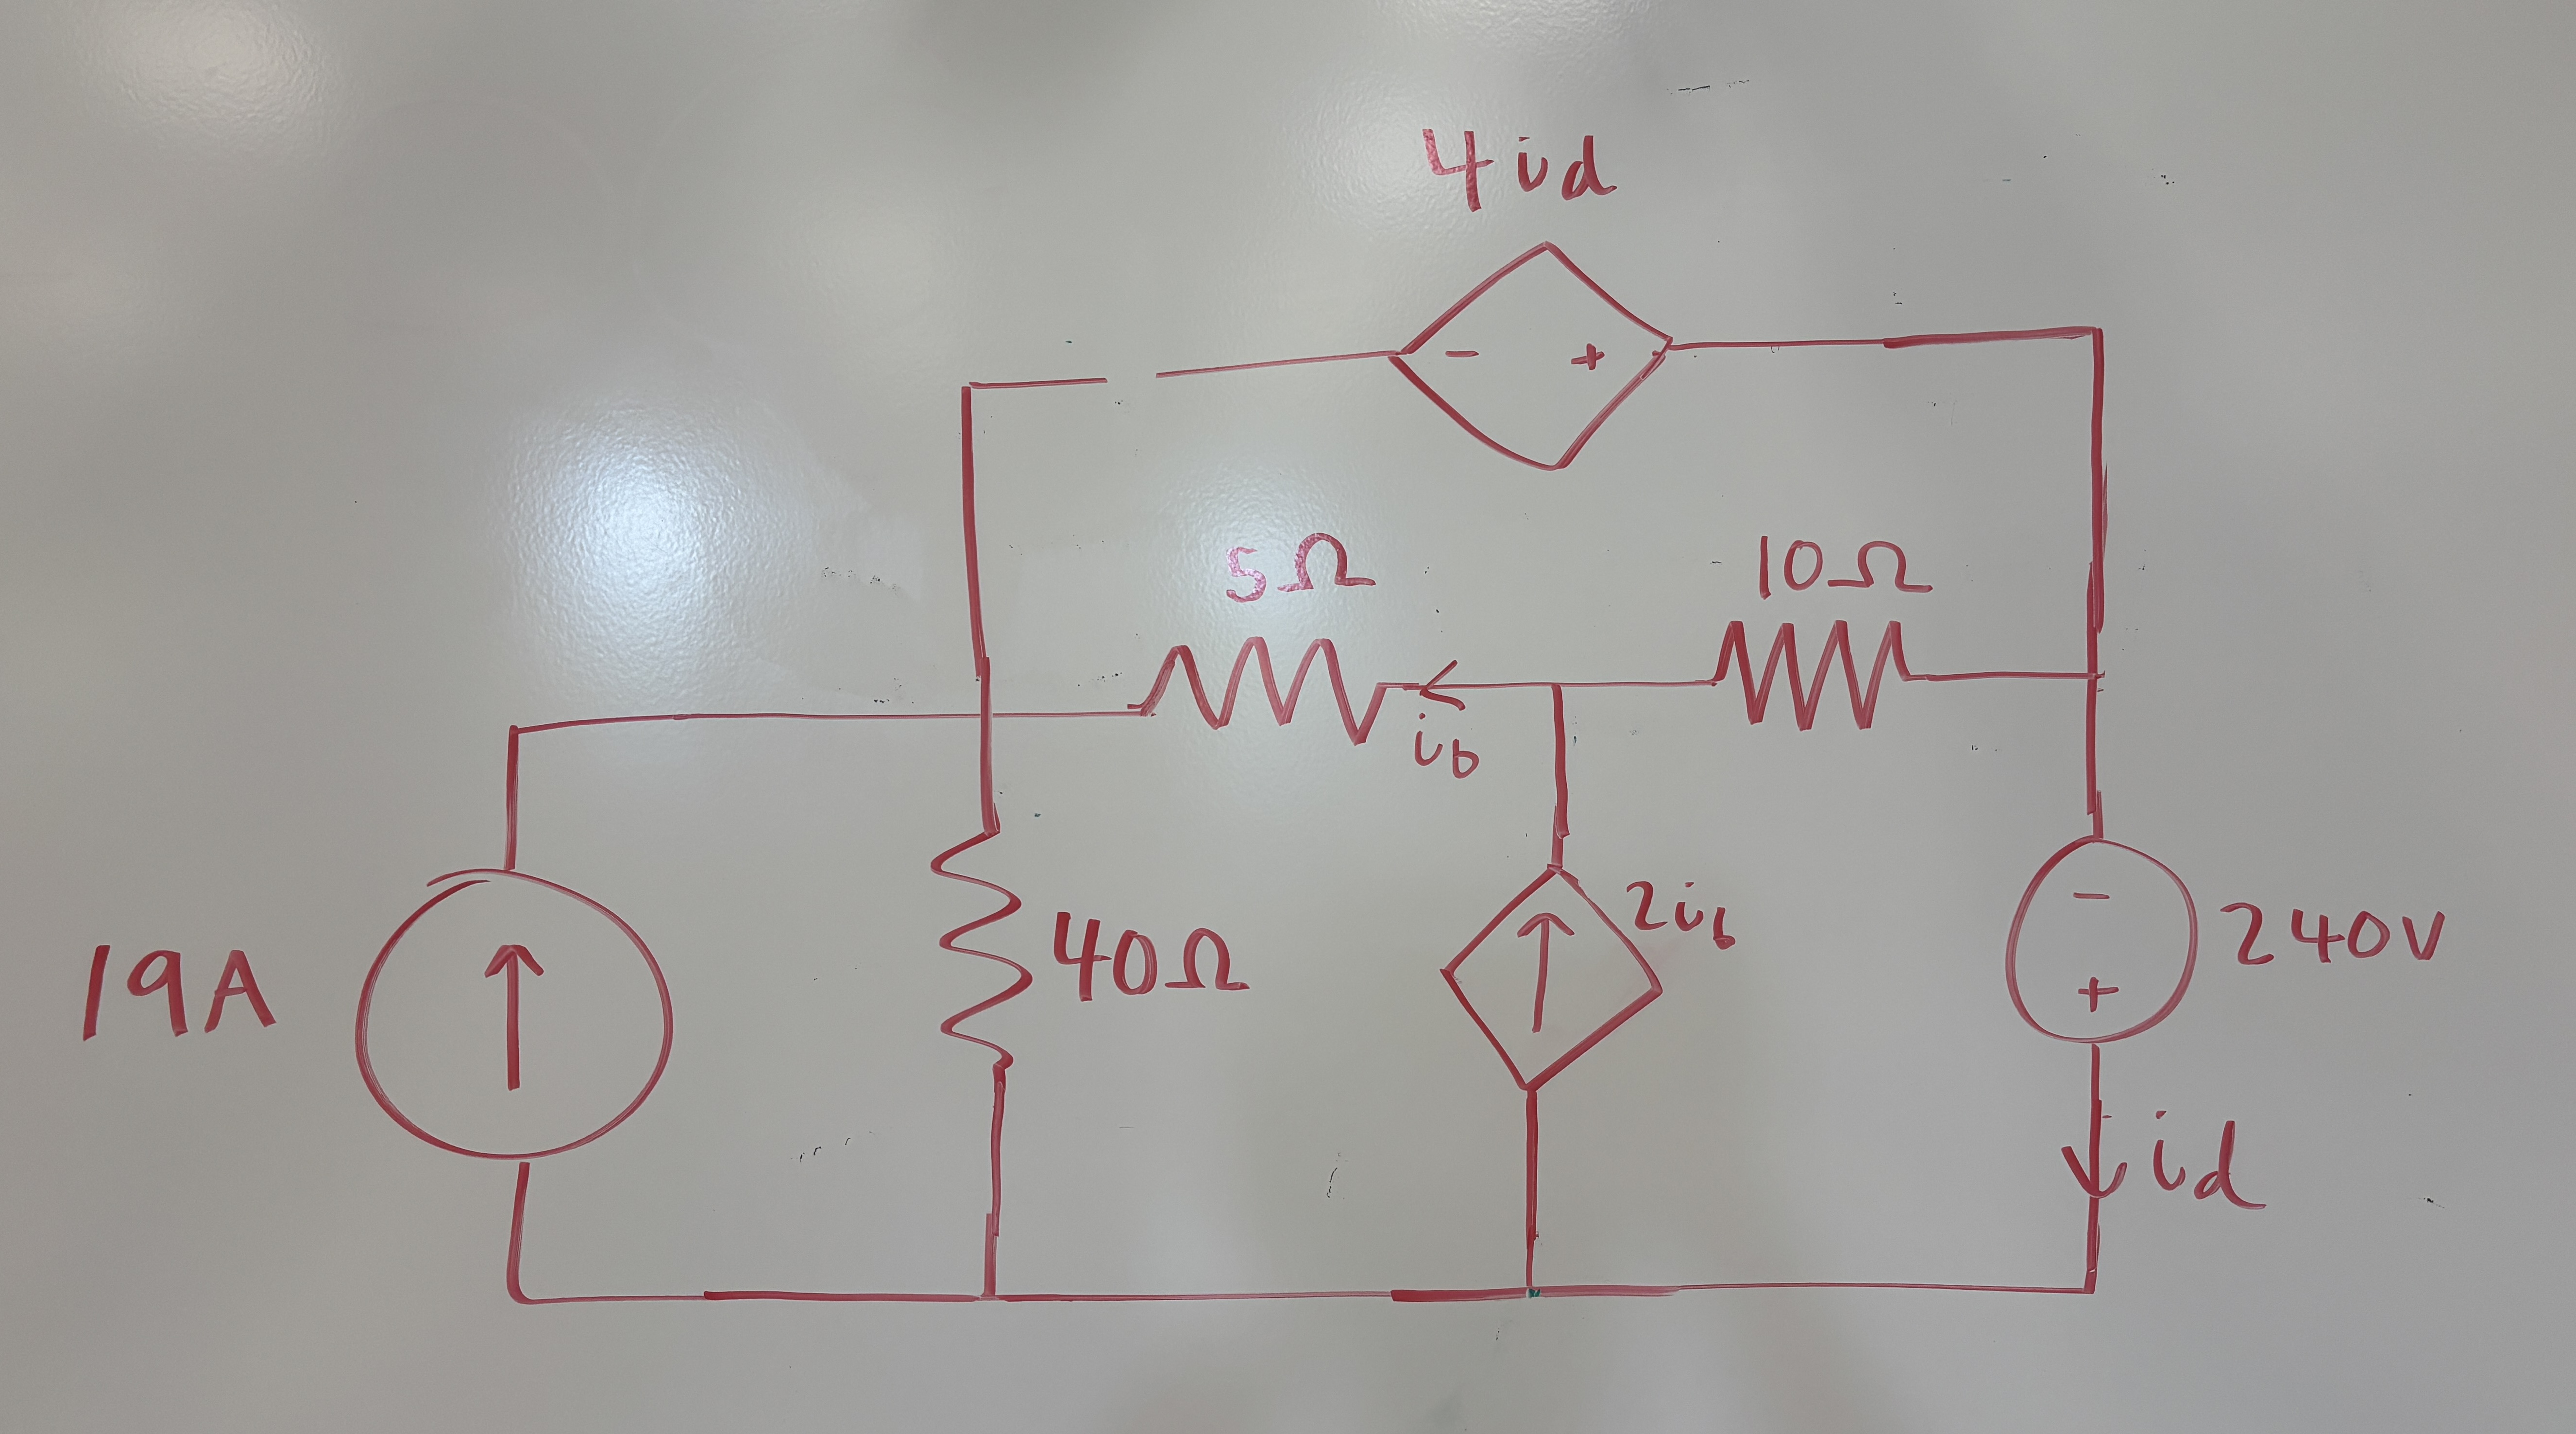
\includegraphics[width=4in]{circuit.jpg}
\end{center}

\begin{partquestion}{solve}{Solve the circuit. Find all voltages and currents.}
\begin{answer}

First thing to do is to assign a node to be ground to establish our variables. Let's call the lowest node ground. This immediately lets us know that the node on the right is at \qty{-240}{\volt}. Let's assign the unknown voltages symbols $V_A$ and $V_B$.

\begin{center}
    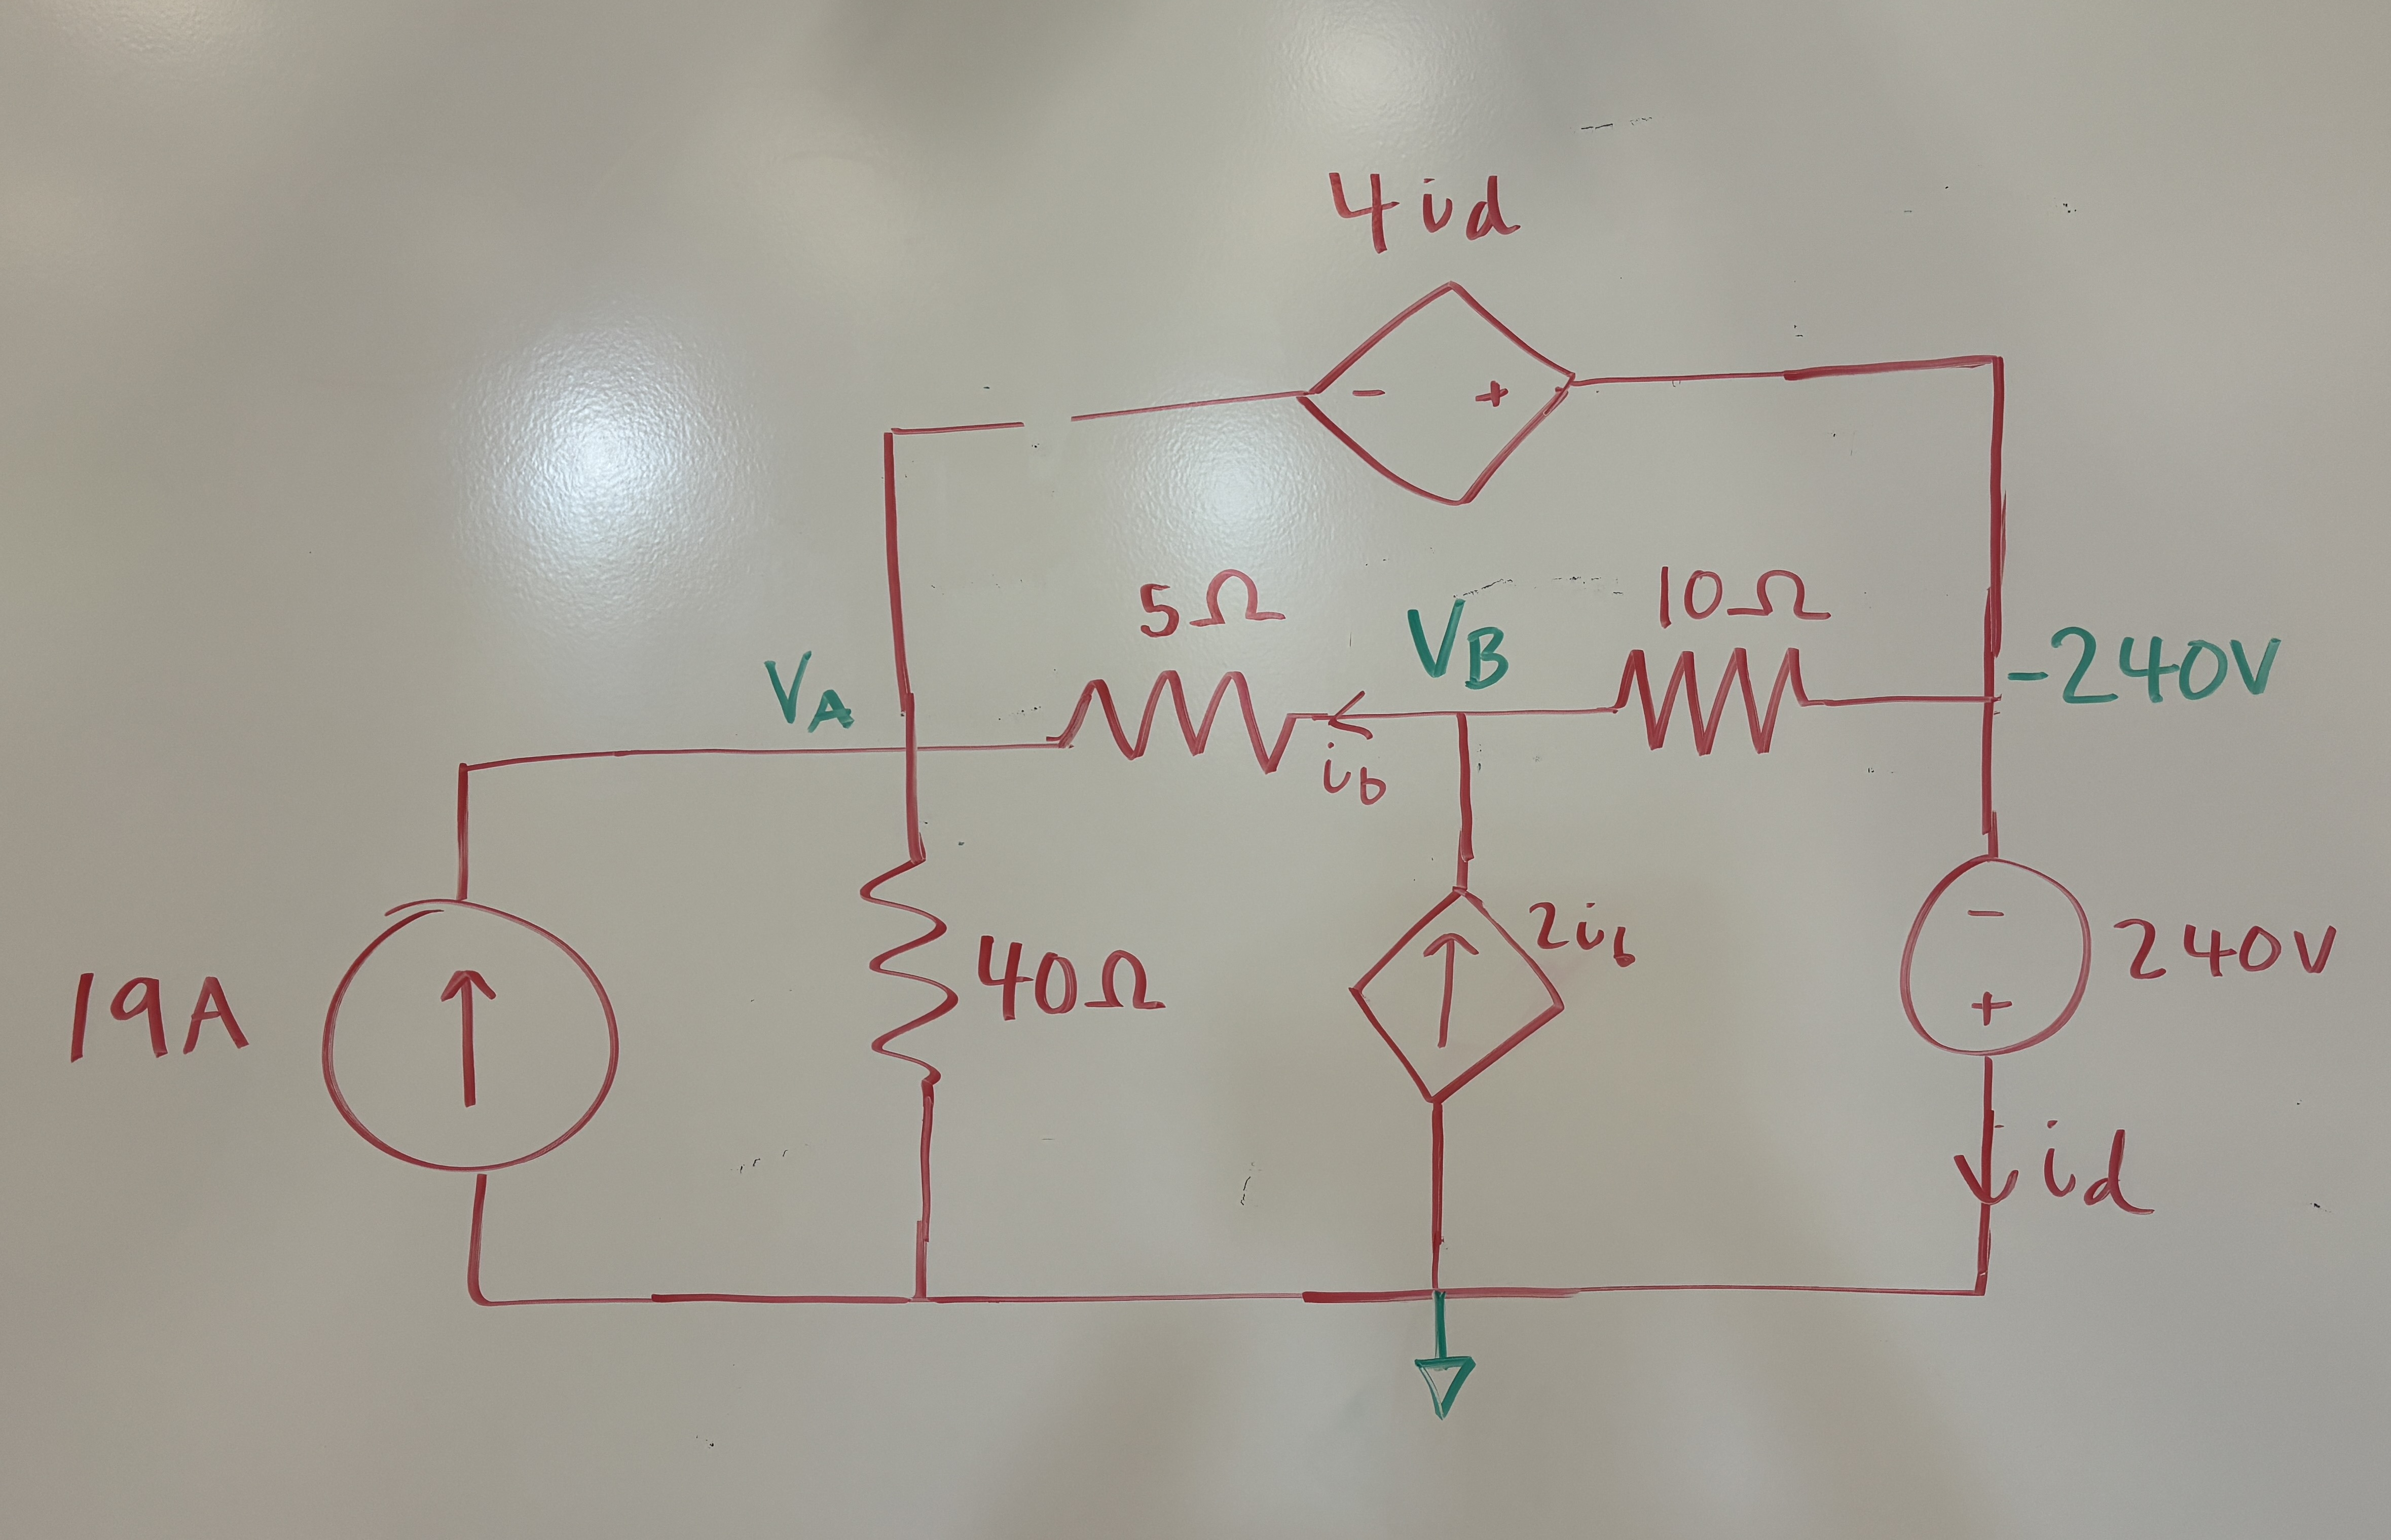
\includegraphics[width=4in]{annotate.jpg}
\end{center}

Now we need to find a set of equations that will let us solve for all the unknowns. We must include an equation for each dependent source. Let's add the KVL equation for the dependent voltage source, and the KCL equation for the dependent current source. Looking at these two equations, we have 4 unknowns. We'll need two more equations that don't introduce any other unknown variables to solve the circuit. Ohm's law at the \qty{5}{\ohm} resistor and KCL at the ground node will do.

\begin{center}
    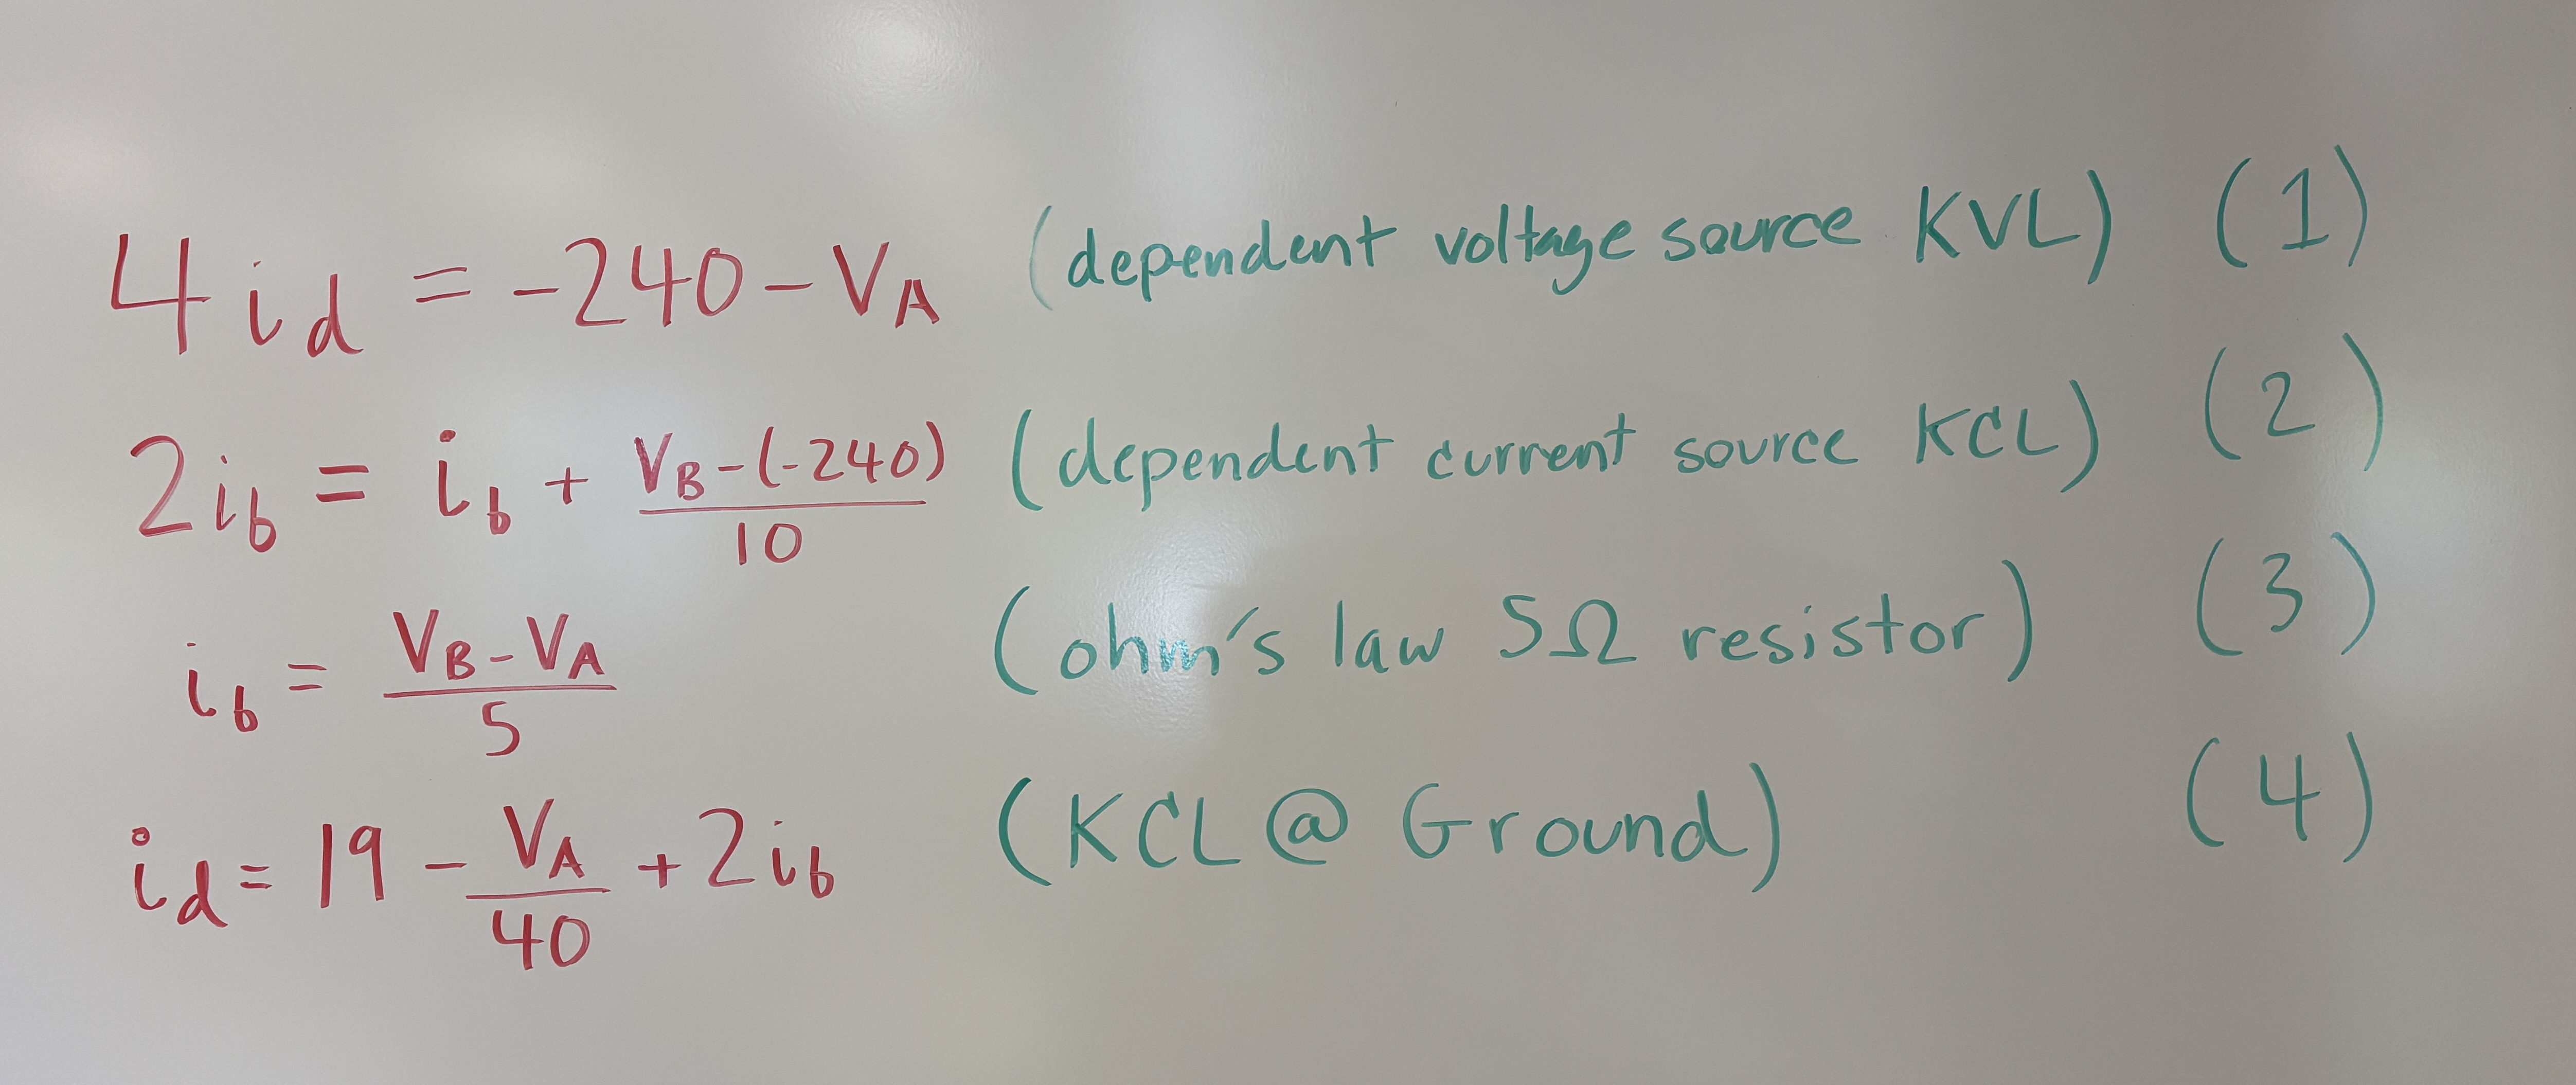
\includegraphics[width=4in]{equations.jpg}
\end{center}

Okay great, let's start combining equations until we have a simple system of 2 equations in terms of $V_A$ and $V_B$.

\begin{center}
    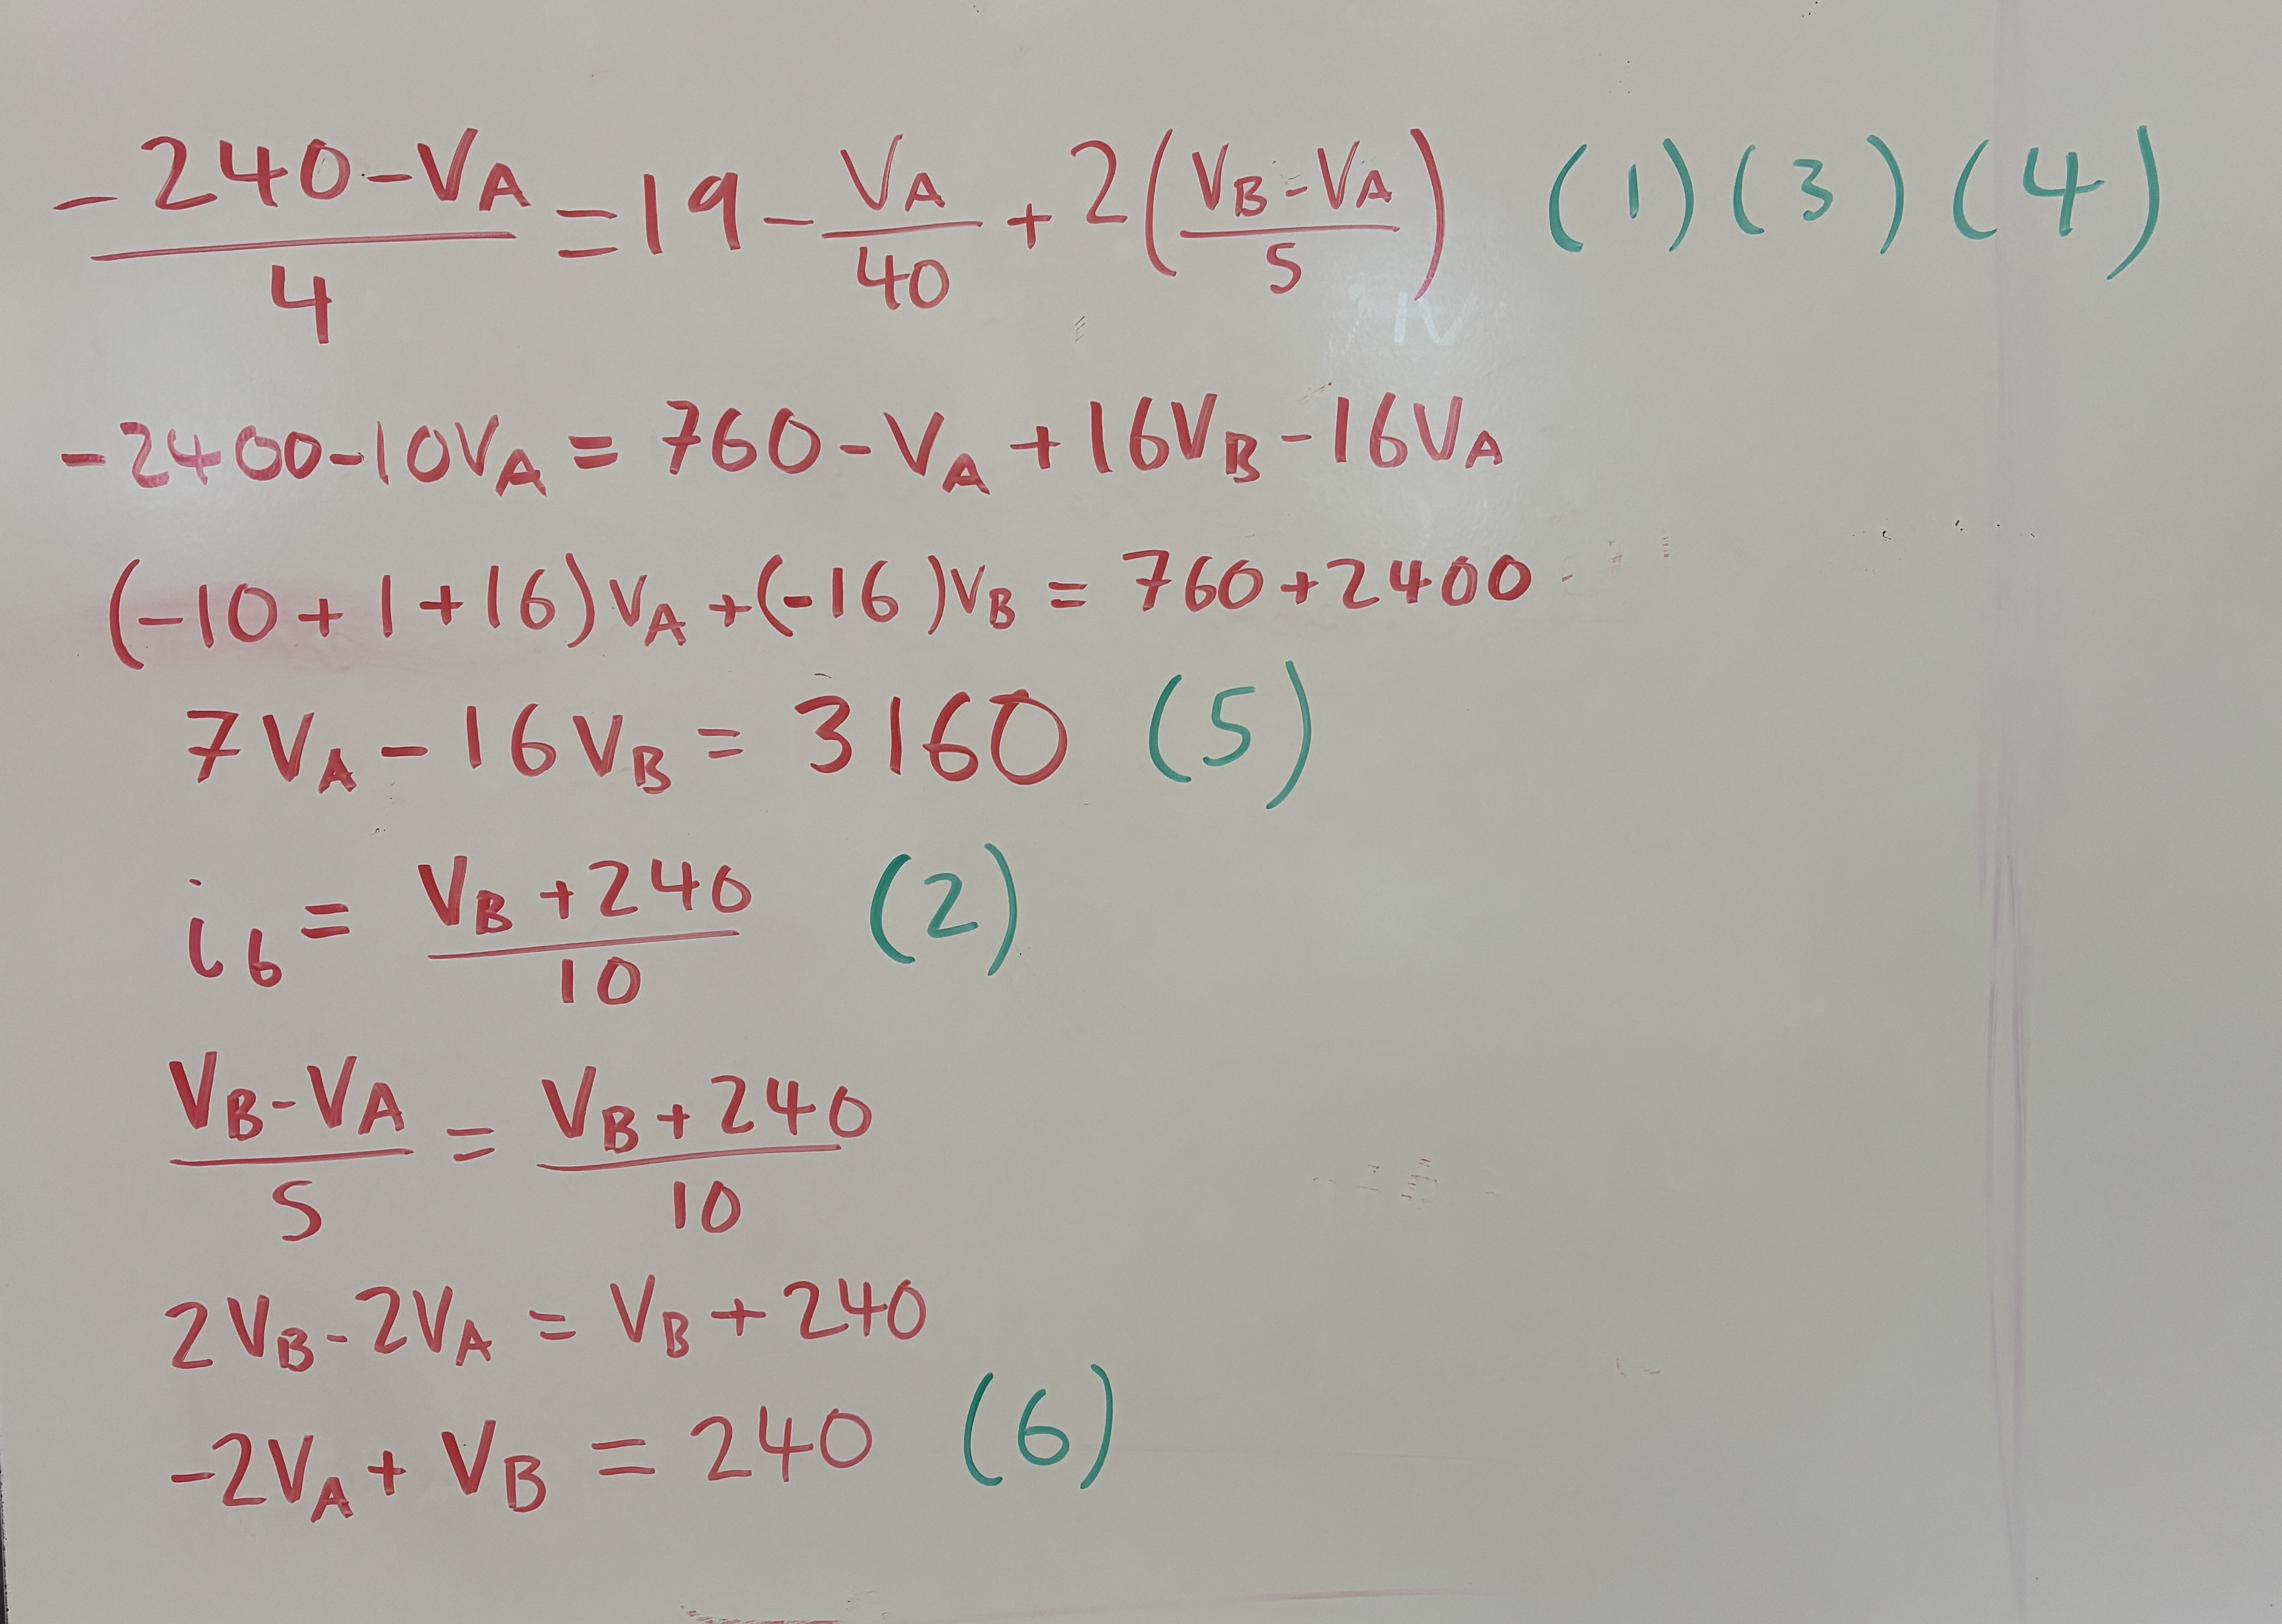
\includegraphics[width=4in]{math.jpg}
\end{center}

Now we solve the system of equations:

\begin{center}
    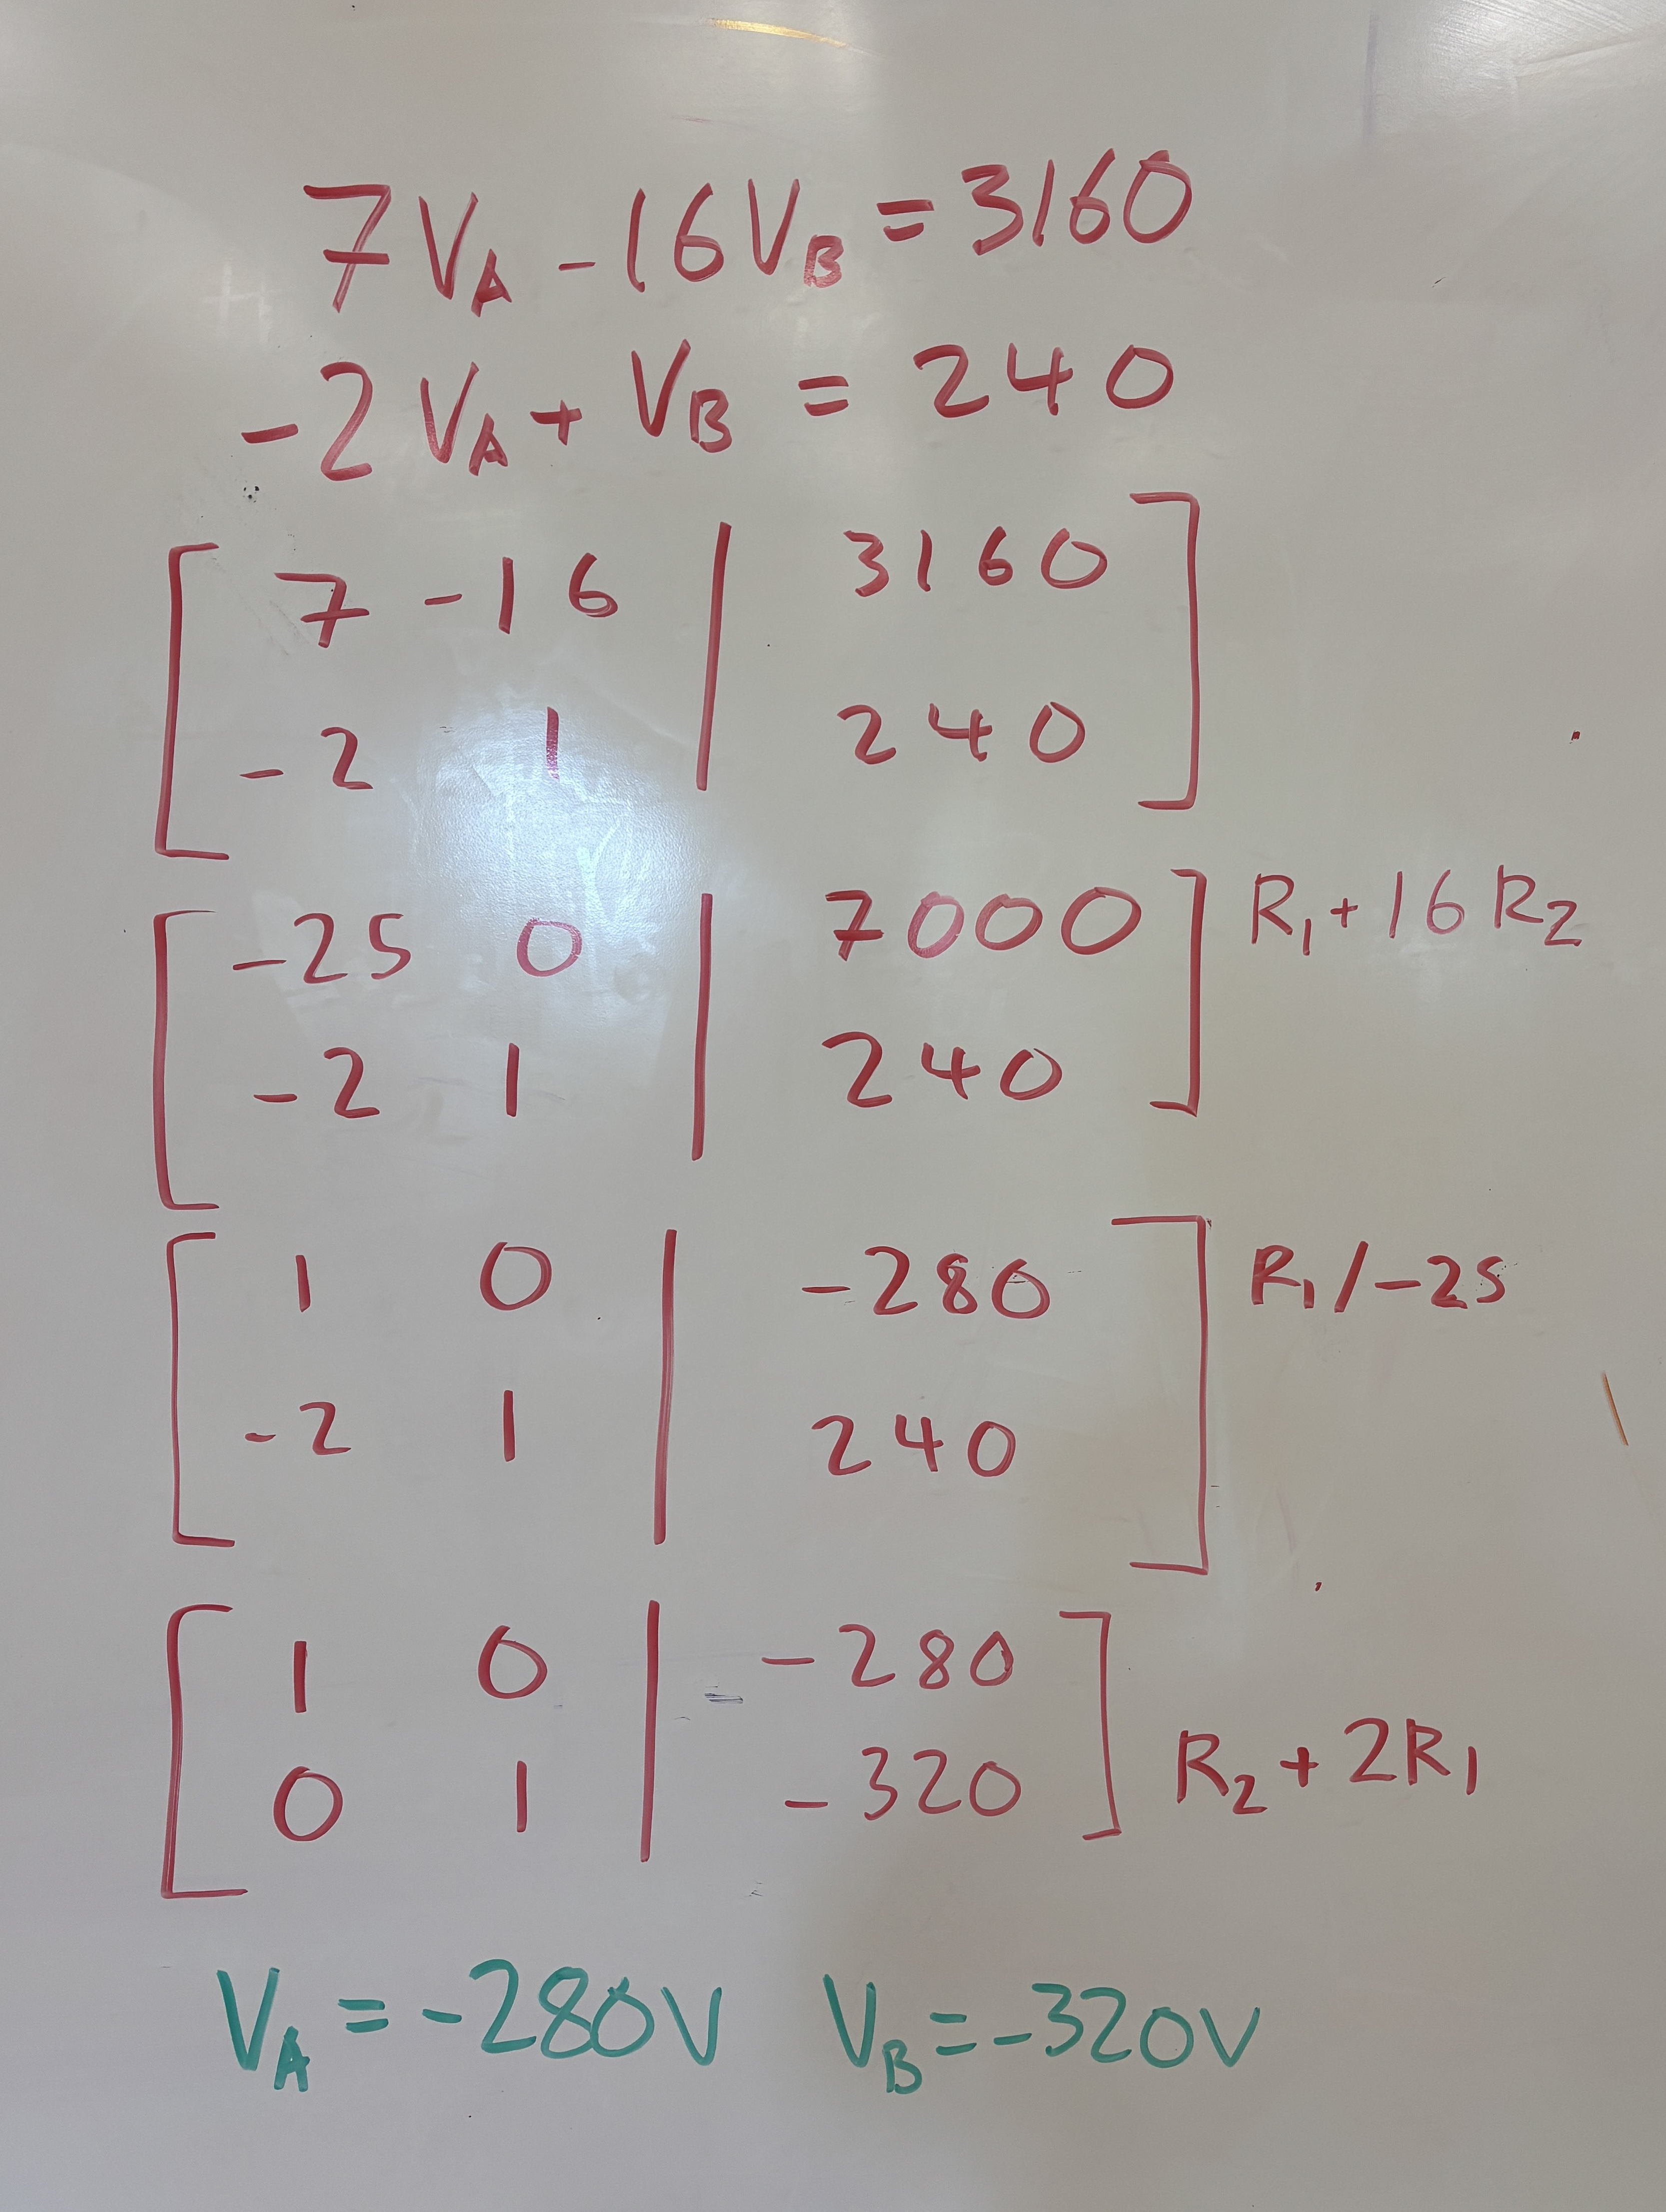
\includegraphics[width=4in]{system.jpg}
\end{center}

These numbers look nice and round, often a good sign if the problem came from a textbook. Let's plug them back into the circuit and verify KCL and KVL hold.

\begin{center}
    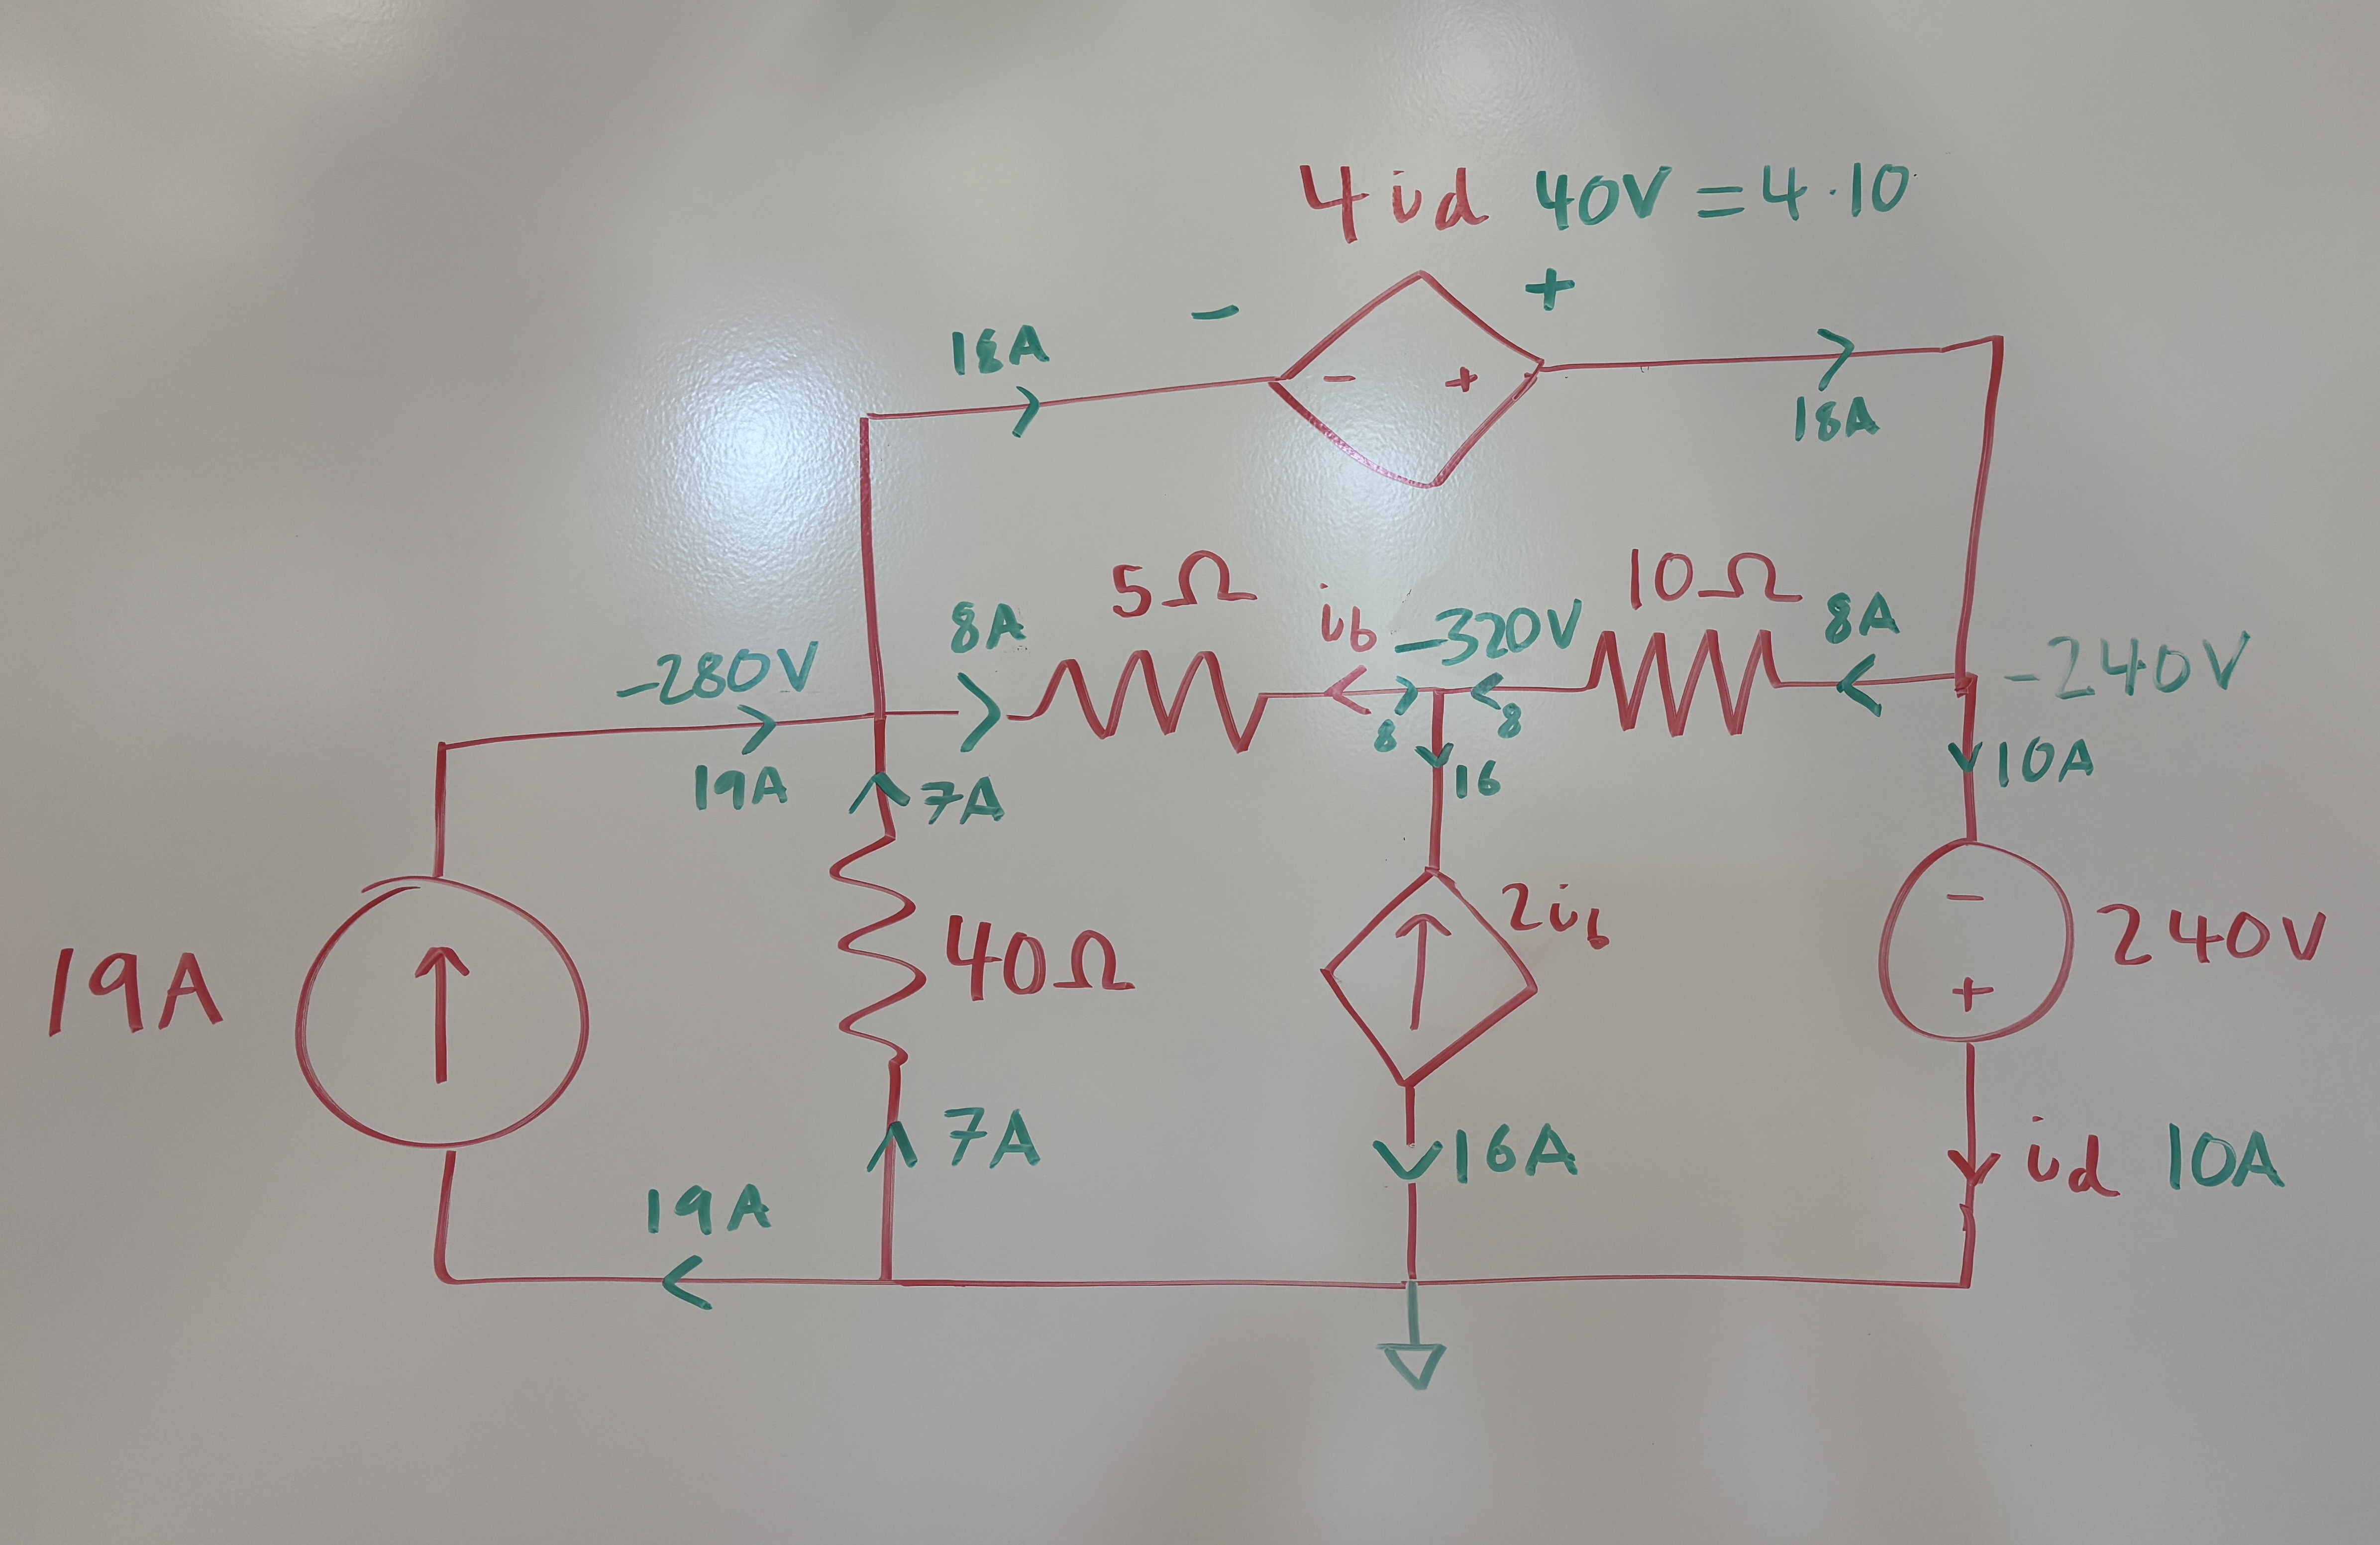
\includegraphics[width=4in]{check.jpg}
\end{center}

Everything looks good! The current entering a node equals the current leaving a node, and the sum of voltages added in a loop is always zero. We've solved the circuit!

\end{answer}
\end{partquestion}

\end{mainquestion}
